
\documentclass[11pt,a4paper]{article} % Paper type (a4paper, usletter or legal) and font size (10, 11 or 12)

\setlength\topmargin{-48pt} % Top margin
\setlength\headheight{0pt} % Header height
\setlength\textwidth{7.0in} % Text width
\setlength\textheight{9.5in} % Text height
\setlength\oddsidemargin{-30pt} % Left margin
\setlength\evensidemargin{-30pt} % Left margin (even pages) - only relevant with 'twoside' article option

\usepackage[sfdefault]{FiraSans} %% option 'sfdefault' activates Fira Sans as the default text font
\renewcommand*\oldstylenums[1]{{\firaoldstyle #1}}
% \usepackage{charter} % Charter font for main content
\usepackage{lmodern}

\frenchspacing % Reduces space after periods to make text more compact for a three-column layout

\usepackage[svgnames]{xcolor} % Enabling colors by their 'svgnames'
\usepackage{graphicx} % Required for including images
\usepackage{amssymb,amsmath} % Math packages
\usepackage{multicol} % Required for the three-column layout of the document
\usepackage{url} % Clickable links
\usepackage{enumitem} % Reduces the amount of space within and between lists with [noitemsep,nolistsep]
\usepackage{marvosym} % Required for the use of symbols
\usepackage{wrapfig} % Allows wrapping text around figures
\usepackage[T1]{fontenc} % Use 8-bit encoding that has 256 glyphs
\usepackage[utf8]{inputenc} % Required for inputting international characters
\usepackage{datetime} % Required for defining a custom date style
\usepackage{wrapfig}
\usepackage{caption}
\newdateformat{mydate}{\monthname[\THEMONTH] \THEYEAR}
% Set a custom date format
\usepackage[pdfpagemode=FullScreen, colorlinks=false]{hyperref}
% Link colors and PDF behavior in Acrobat
\usepackage{fancyhdr} % Required to define custom headers/footers
\pagestyle{fancy} % Enables the custom headers/footers for all pages following this

\usepackage{geometry} % Required for adjusting page dimensions

\geometry{
	top=1cm, % Top margin
	bottom=1.5cm, % Bottom margin
	left=2cm, % Left margin
	right=2cm, % Right margin
	includehead, % Include space for a header
	includefoot, % Include space for a footer
	%showframe, % Uncomment to show how the type block is set on the page
}


%-----------------------------------------------------------
% Header and footer
\lfoot{
}

\cfoot{} % Empty center footer

\rfoot{\footnotesize ~\\ Page \thepage} % Right footer - page counter

\renewcommand{\headrulewidth}{0.0pt} % No horizontal rule for the header
\renewcommand{\footrulewidth}{0.4pt} % Horizontal rule separating the footer from the document
%-----------------------------------------------------------

%-----------------------------------------------------------
% Define separators
% \newcommand{\HorRule}[1]{\noindent\rule{\linewidth}{#1}}
\newcommand{\HorRule}{\color{DarkGoldenrod}\rule{\linewidth}{1pt}} % Defines the gold horizontal rule around the title
% Creates a horizontal rule
\newcommand{\SepRule}{\noindent % Creates a shorter separator rule
    \begin{center}
        \rule{250pt}{1pt} % Page width and rule width
    \end{center}
}
%-----------------------------------------------------------

%-----------------------------------------------------------
% Define title and article styles
\newcommand{\NewsletterName}[1]{ % Newsletter title
    \begin{center}
        \Huge \usefont{T1}{fvs}{b}{n} % Use the Bera Sans Bold font
        #1
    \end{center}
    \par \normalsize \normalfont}

\newcommand{\JournalIssue}[1]{ % Date and issue number at the top of the newsletter
    \textsc{Physics World}\hfill \textsc{\mydate \today, No #1} % Right-aligned date and issue number
    \par \normalsize \normalfont}

\newcommand{\NewsItem}[1]{ % News item title
    % \usefont{T1}{fvs}{n}{n} % Use the Bera Sans Normal font
    \vspace{24pt} \large \textbf{#1}\vspace{5pt} % Print the title with space around it in a larger font size
    \par \normalsize \normalfont}

\newcommand{\NewsAuthor}[1]{ % Author name under the item title
    \hfill by \textsc{#1} \vspace{20pt} % Right-aligned author name in small caps with space after it
    \par \normalfont}

\newenvironment{Figure}
  {\par\medskip \noindent\minipage{\linewidth}}
  {\endminipage\par\medskip }

%----------------------------------------------------------------------------------------
%	TITLE SECTION
%----------------------------------------------------------------------------------------

\newcommand{\authorstyle}[1]{{\large\usefont{OT1}{phv}{b}{n}\color{DarkRed}#1}} % Authors style (Helvetica)

\newcommand{\subtitlestyle}[1]{{\centering\Large\usefont{T1}{lmss}{m}{it} #1 \par}}

\usepackage{titling} % Allows custom title configuration
\usepackage{changepage}


\pretitle{
    \JournalIssue{4} % Issue number
	\vspace{-10pt} % Move the entire title section up
	\HorRule\vspace{10pt} % Horizontal rule before the title
    \begin{center}
        \vspace{10pt}
        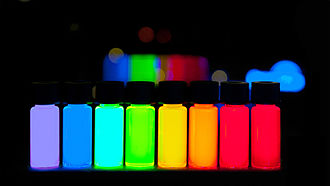
\includegraphics[width=0.6\linewidth]{330px-Quantum_Dots.jpg}
        % \par\large\textit{An interesting caption to this drab picture\ldots}
        \vspace{10pt}
    \end{center}
	% \fontsize{32}{36}\usefont{OT1}{phv}{b}{n}\selectfont % Helvetica
    \fontsize{32}{36}\usefont{T1}{lmss}{b}{n}
	\color{Black} % Text colour for the title and author(s) (original: DarkRed)
    \centering
}

\posttitle{ \par\vskip 15pt % Whitespace under the title
            \begin{adjustwidth}{1cm}{1cm}
            \subtitlestyle{
                A new generation of display technology using the powerful abilities of
                quantum physics will enter the markets soon.
                }
            \end{adjustwidth}
            }

\preauthor{ \begin{flushright}} % Anything that will appear before \author is printed

\postauthor{ \end{flushright}
    % Anything that will appear after \author is printed
	% \vspace{10pt} % Space before the rule
	% \par\HorRule % Horizontal rule after the title
	\vspace{-40pt} % Space after the title section
}

\title{Will Quantum Dots be Relevant in Future Displays?}
% The article title

\author{
	\authorstyle{by somebody}
	% \textsuperscript{1}\institution{Universidad Nacional Autónoma de
	% 	México, Mexico City, Mexico}\\ % Institution 1
}
\date{}


% \usepackage{tikz,lipsum,lmodern}
\usepackage[most]{tcolorbox} 

\usepackage[natbib=true,backend=biber,style=phys,citestyle=phys%,%
%sorting=ynt%
]{biblatex}

\usepackage{csquotes}

\addbibresource{tex/references.bib}

\begin{document}

% \NewsletterName{Newsletter Title} % Newsletter title
\maketitle

% \noindent\HorRule{3pt} \\[-0.75\baselineskip] % Thick horizontal rule
% \HorRule{1pt} % Thin horizontal rule
%----------------------------------------------------------------------------------------
%	MAIN NEWS ITEM
%----------------------------------------------------------------------------------------

% \vspace{0.5cm}
% \SepRule
% \vspace{-0.5cm}

%\setlength{\columnsep}{16pt} % Uncomment to manually change the white space between columns
\begin{multicols}{2} % Begin the three-column layout

    One thing is sure. Our digitalised world wouldn’t be possible without
    displays and the demand for energy efficient, cheap and realistic
    presentation
    of information is higher than ever. The most successful display
    technologies
    currently on the market are LCD and OLED displays but tech companies like
    Samsung already started to introduce so called QLED TV’s. Sounds close to
    OLED
    you might think, but the difference is more fundamental than the name
    suggests.
    The new technology here is the use of so called Quantum Dots to improve
    colour
    purity, efficiency and many other things.

    Lets dive quickly into the relevant physics.
    % A quantum dot is a piece of
    % semiconductor, for example cadmium selenide (CdSe), that is so small (in
    % the range of nanometres) that the energy levels of electrons inside it
    % change
    % significantly from a large piece.
    % If an electron of a higher energy state changes into a lower energy state,
    % the energy difference is emitted as light of a certain colour. The change
    % of
    % the energy states in quantum dots can be understood well enough to create
    % materials that can emit almost any color [ElectronElectronBrus].
    % So, to produce a colour from a quantum dot one only needs to introduce
    % excited electrons and corresponding free states in the quantum dot.
    In semiconductors there is a range of energies the electrons can’t have,
    the so called band gap. This band gap usually separates the mostly filled
    energy states which are the valence electrons that bind the atoms of the
    material and the higher and mostly empty energy states of conducting
    electrons.
    These energy states are also called valence band and conduction band. 
    
    A  quantum dot is a spherical piece of semiconductor, for example cadmium
    sulfide (CdS), with a size in the range of nanometres. In that regime its 
    band gap changes significantly from its initial value. For example in the case of
    CdS, which typically has a band gap of 2.6eV the band gap can be increased up to
    3.5eV \cite{Brus1998}.

    If an electron of a higher energy state changes into a lower energy state,
    the energy difference is emitted as light of a certain wavelength $\lambda$
    given by $E=\frac{h}{\lambda}$. By varying the size of the quantum dots it
    is possible to create	materials that can emit almost any colour \cite{Brus1998}.

    \NewsItem{What a Display should have}
    Our eye perceives colour over so called cones, sensors for red, green and
    blue light. An ideal display matches our natural perception of objects by
    transmitting a mixture of these three colours. 
    
    %####
    The set of colours a display
    can
    represent is the colour gamut that can be represented in the so called CIE
    1931
    chromaticity diagram shown in figure \ref{fig:CIEchrom}. Colours close to the edge have
    single wavelengths and going to the middle we find mixtures of these
    colours.
    The gamut of a display is represented by the area of the triangle between
    the
    three primary colours. The wider the gamut the more
    colourful
    display seems to us.
%########## more colorful
    Quantum dots emit light with very narrow peak widths compared to typical
    organic emitters in OLEDs or color spectra from lcd screens. This makes it
    possible to achieve much wider gamuts than currently on the market.

    
    \begin{tcolorbox}[colback=red!5!white,colframe=red!75!black]
        \subsection*{The Color Gamut}
        The color gamut is the subset of all colors a display can
        produce from three primary colors. A comparison of the 
        QD-LCD gamut with current industry standards like Rec 2020
        and NTSC in the so called CIE 1931 xy chromaticity diagram is 
        shown below.
        \begin{center}
            \vspace{10pt}
            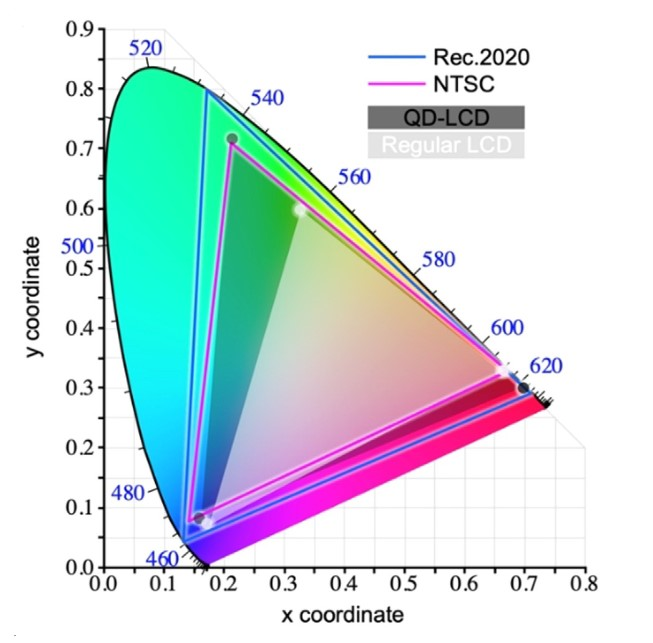
\includegraphics[width=0.8\linewidth]{ColorGamut2.jpg}
            \captionof{figure}{}
            \label{fig:CIEchrom}
            \vspace{10pt}
        \end{center}
    \end{tcolorbox}

    Other factors of consideration are also the brightness of the display and
    its operational lifetime.

    %-----------------------------------------------------------

    \NewsItem{How to Use a Quantum Dot}
    This mechanism can be implemented into displays in two different ways. The
    first way is the down conversion of blue light into green and red light,
    also called photoluminescence. The incoming blue photon excites an electron
    over
    the band gap. Usually, the photon doesn’t recombine directly but loses
    energy
    to the semiconductor lattice until it reaches the band gap. From there it
    recombines with a free electron state it created and emits a photon of
    the colour corresponding to the band gap width.

    The colour gamut of  LCD screens, which work on a white backlight with
    colour filters for red and green colour can be improved significantly by
    using quantum dots. In a first step currently marketed by Samsung as QLED TV’s
    \cite{ctarticle} ,
    a blue LED light source is combined with a layer of colloidal quantum dots
    for
    green and red colour instead of yellow phosphor. This makes possible a wide
    colour gamut but can only be an intermediate solution. The light source
    still
    creates much more light than is used in the end for the creation of the
    picture
    \cite{Shu2020}. Also, the contrast, the maximal difference between pixels
    on the screen in brightness on the screen
    is limited by the remains of backlight coming through switched off pixels.
    This is a large disadvantage to OLED screens which can switch of pixels
    completely
    and thus also save additional power\cite{Brus1998}% \cite{Liu2020}.

    \begin{Figure}
        \centering
        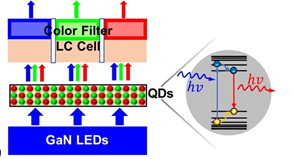
\includegraphics[width=0.9\linewidth]{photolumLED.png}
        \captionof{figure}{LCD pixel with QD enhanced backlight}
    \end{Figure}

    A different approach using photoluminescence is to exchange the backlight
    by µLED’s for each pixel to fix the disadvantage in contrast compared to OLED.
    The µLED’s emit blue light that is then converted to green and red light by
    quantum dots directly in the pixel. The challenges with this method are the so
    called cross talk, the lighting of deactivated pixels by neighbouring LED’s and
    remaining blue light in pixels with different colours. These effects can be
    controlled by introducing additional light barriers and altering parameters,
    but make the fabrication process more expensive.

\end{multicols}

\begin{tcolorbox}[colback=red!5!white,colframe=red!75!black]
    \begin{minipage}{0.45\textwidth}
        \subsection*{LCD vs OLED Structure}
        The fundamental difference between LCD and OLED is the creation of colours.
        In a LCD a white backlight is filtered to get the colour of each subpixel 
        while an OLED uses the electronic energy levels of special organic materials
        to create the color for each subpixel.
    \end{minipage}
    \hspace{15pt}
    \begin{minipage}{0.45\textwidth}
    \begin{center}
        \vspace{10pt}
        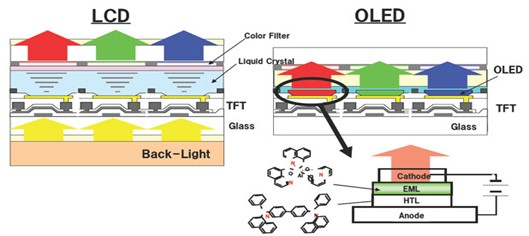
\includegraphics[width=\linewidth]{OldConcepts.jpg}
        \captionof{figure}{taken from \cite{overwievpicture}}
        \label{fig:CIEchrom}
        \vspace{10pt}
    \end{center}
\end{minipage}
\end{tcolorbox}

\begin{multicols}{2}

    On the other hand, this approach can combine a wide colour gamut and high
    contrast which removes the major disadvantages of LCD displays and outperforms
    current OLED’s. It shows also a higher stability in brightness and colour over
    time and environmental changes that trouble OLED TV’s. Even largest problem of
    OLED’s, the so called “burn in” of frequently shown patterns with on the same
    set of pixels doesn’t occur on those QD-µLED TV’s because their lifetime is
    significantly larger \cite{Liu2020}.

    Although all this sounds very promising, there is a lot of engineering
    involved to improve photoluminescent quantum dot displays which makes them more
    expensive. A different physical approach to create light from quantum dots is
    by electroluminescence, which lets them emit light without another primary
    light source. The colloidal quantum dots are placed between two semiconductor
    layers as seen in figure \ref{fig:QDLED} which supply free electrons from one side, the
    electron transport layer (ETL), and so called holes from the other side, the
    hole transport layer (HTL). Holes are not occupied electron states in an
    environment of occupied states. It is possible to model them as particles with
    positive electron charge. Through that setup, holes and electrons recombine in
    the quantum dot, emitting light with band gap energy.

    \begin{Figure}
        \centering
        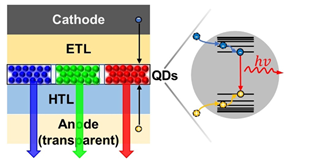
\includegraphics[width=0.9\linewidth]{ellumLED.png}
        \captionof{figure}{QD-LED pixel}
        \label{fig:QDLED}
    \end{Figure}

    This concept promises to be even better than the other methods presented so
    far. Light of a certain colour is only emitted when needed which saves a
    significant amount of energy and the high contrast ratio of µLED and OLED
    screens can be maintained. Saving energy equivalently also means potential
    higher brightness \cite{ctarticle}. The ability to process Quantum Dots dispersed
    in a polymer enables to use established production methods and
    the relatively simple structure of QLED TV’s is also likely to lead to cheaper
    production costs than current OLED’s.

    % \end{multicols} % End the three-column layout for a large picture

    % \begin{wrapfigure}{l}{0.4\linewidth}
    %     \centering
    %         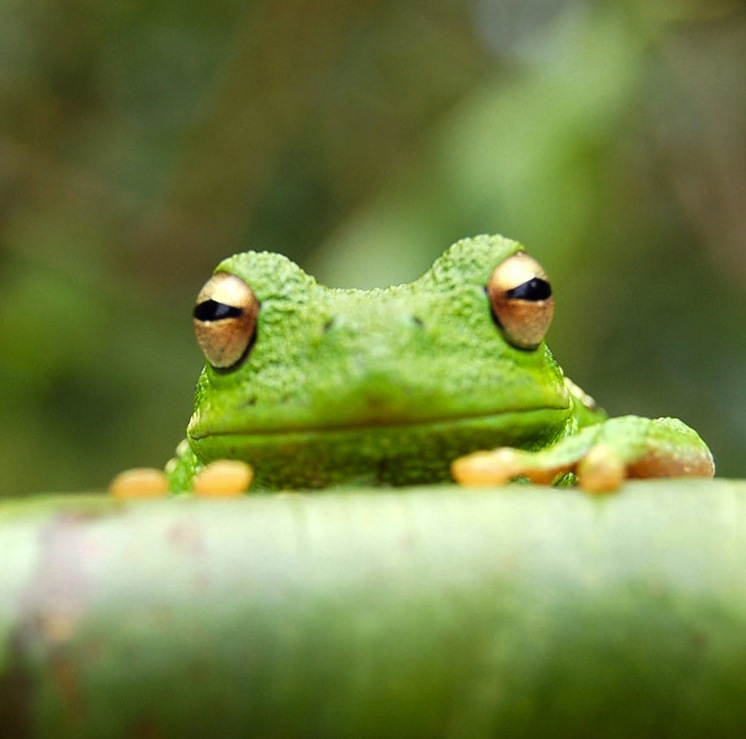
\includegraphics[width=0.6\linewidth]{frog.jpg}
    %     \end{wrapfigure}

    % \begin{center}
    %     \vspace{10pt}
    %     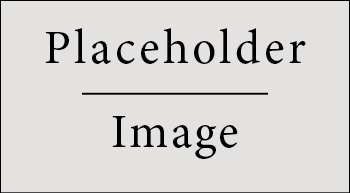
\includegraphics[width=0.8\linewidth]{placeholder.jpg}
    %     % Example of an image taking up the total width of the page
    %     \par\large\textit{An interesting caption to this drab picture\ldots}
    %     \vspace{10pt}
    % \end{center}
    % \begin{figure*}[t]
    %     \centering
    %     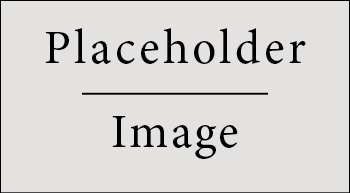
\includegraphics[width=0.7\linewidth]{placeholder.jpg}
    %     \caption{\textit{An interesting caption to this drab picture\ldots}}
    % \end{figure*}

    % \begin{multicols}{2} % Continue the three-column layout

    %-----------------------------------------------------------

    \NewsItem{The Problem with Heavy Metals}
    A major problem for implementing Quantum Dots still remains. The
    semiconductors used for creating light in the optical spectrum involve heavy
    metals like Cadmium in CdSe. These are usually heavily regulated by
    governments. However, for the current Quantum Dot TV’s it was possible to
    reduce the heavy metal concentrations below the set thresholds \cite{Shu2020}. Another
    way would be to use different materials. InP could replace CdSe for red and
    green Quantum dots. In fact, Indium is a regulated heavy metal too, but it is
    allowed in much higher concentrations. The only problem with replacing Cadmium
    completely by Indium would be the creation of blue Quantum dots. Here, a
    solution still needs to be found.

    Overall, we see that the use of Quantum Dots can significantly improve the
    weaknesses of our current technology including OLED TV’s. I’m sure we will see
    more of these in near future.

    % \begin{wrapfigure*}
    %     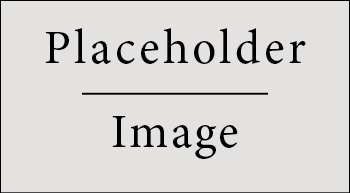
\includegraphics[width=0.9\textwidth]{placeholder.jpg}
    % \end{wrapfigure*}

    % \begin{quotation} % Example of a quotation
    %     \noindent{\Huge``}

    %     \noindent\normalsize\textit{Donec non nisl a arcu consequat varius. Sed
    %         suscipit cursus luctus. Nulla sit amet elit augue. Curabitur
    %         scelerisque mollis
    %         dolor, quis blandit lorem condimentum at.}

    %     \hfill{\Huge''}

    %     \hfill-- John Smith
    % \end{quotation}

\end{multicols}

%----------------------------------------------------------------------------------------
% \newpage
\printbibliography[heading=bibintoc]
\end{document}